\chapter{Data Acquisition and Preprocessing}
    \label{MRIdata}
Before being able to model the cross-sections, reliable anatomical data is needed to base the exact shape on. The way we chose to get the described data is magnetic resonance imaging (MRI). This chapter first sets out the details of the acquisition of the MRI data to then give details about the pre-processing that has been done in order to be able to apply the theoretical model described in the previous chapter.


\section{Acquisition}
    \label{MRI}

For magnetic resonance imaging, we acquired a recently expired but undamaged specimen. The animal was killed for a procedure the preceding day and has been stored refrigerated in partially distilled water. The MRI data was acquired using a 3T clinical scanner (Prisma Fit, Siemens Healthineers AG, Erlangen, Germany) equipped with a flexible 4-canal wrapped-around coil (Flex Small, Siemens Healthineers AG, Erlangen, Germany) and a maximal gradient strength of 80 mT/m. Applying the spin-echo technique, we could get two types of sections useful for modelling purposes: paramedian and paratransverse sections. Paramedian pictures were created using a field-of-view (FOV) of $192 \times 36 \times 24$ mm and a resolution of $0.3 \times 0.3 \times 0.6$ mm, paratransverse pictures with a FOV of $38 \times 27 \times 128$ mm and a resolution of $0.15 \times 0.15 \times 1$ mm. Examples of both types are illustrated in Figure \ref{MRIpic}.

The paramedian pictures are not informative for the shape of the cross-sections but rather give an idea about the location of the backbone, the spinal chord and the electric organ. The latter is placed within the marked red box in Figure \ref{paramedian} while the backbone, detectable by the repeated changes between dark and bright, is located dorsal to it inside the yellow box. In the paratransverse sections the backbone is visible until the cranial end of the swim bladder. Still, in the paramedian picture it cannot be detected till this point. That is why it is only marked until where it is visible in the paramedian data. The pairic structure of \textit{A. Leptorhynchus'} electric organ results from its neurogenicity \cite{bennett1971electric} that is unique for this species, as far as we know. Even further dorsal to the backbone, one can find the spinal chord not clearly visible in the depicted paramedian section, though. The illustrated cross-section on the contrary shows the spinal chord marked in blue quite well. 

\begin{figure}
\begin{tcolorbox}
\centering
\begin{subfigure}[b]{1\textwidth}
    \centering
   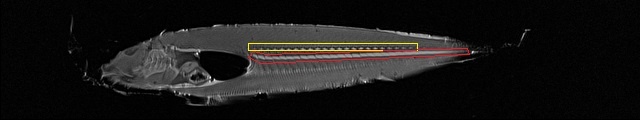
\includegraphics[width=1\linewidth]{figures/coronal_marked.jpg}
   \caption{}
   \label{paramedian} 
\end{subfigure}

\begin{subfigure}[b]{1\textwidth}
    \centering
   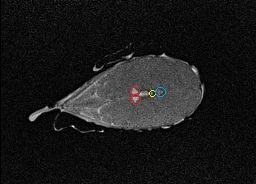
\includegraphics[width=0.5\linewidth]{figures/transverse_marked52.jpg}
   \caption{}
   \label{paratransverse}
\end{subfigure}
\end{tcolorbox}

\caption{MRI data from \textit{Apteronotus Leptorhynchus}. The electric organ is marked in red, the fish's backbone in yellow, and the spinal chord is marked in blue. \textbf{a)} Paramedian section close to the median plane (20 mm from the fish's left). \textbf{b)} Paratransverse section located caudal to the swim bladder (52 mm caudal to the fish's head).}
\label{MRIpic}
\end{figure}

A procedural error in specimen transition to the final measurement configuration lead to artifacts induced by
residual water in the plastic container. This noise is visible in Figure \ref{paratransverse} as grey points or lines around the cross-section itself. Its color made image processing without editing impossible as edge detection has been one of the first necessary steps in that process and the noise was detected as edges as well. Hence, preprocessing of the MRI-cross-sections has been done in form of removing all grey pixels around the fish's body. As this has been executed by hand, it may have led to some inaccuracies in the outer contour of the cross-sections because fish and bag are not always clearly distinguishable. Another consequence was the exclusion of the first eight sections from the editing and thus from the whole modelling process, because bag and fish were not to be distinguished.

Furthermore, the backbone's position needed to be marked in the MRI pictures to be later able to parameterise the cross-section's position relative to it. That was done via coloring the pixels considered as being located inside the backbone in fullwhite by hand, as well. Due to time limits this editing process has only been applied to half of the cross-sectional MRI data. Additionally, we evaluated 60 pictures as being an exact enough basis for later regressions and approximations.

\section{Preprocessing}
    \label{preprocessing}
    
To parameterise the single cross-sections as described in section \ref{Cross sections}, it is obligatory to first determine each contour's distance to the backbone depending on the point on the backbone $l$ and the angle $\varphi$. This can only be done after having transformed and edited the MRI data in various ways. The steps we have executed in order to calcute the mentioned distances are explained in the following paragraphs. 

As a first step, the edited MRI cross-sections were imported into the python project as grey-scale images. To exclude all unneccessary remaining noise outside the fish's contour, a canny edge detection \cite{canny1986computational} has been executed. It uses a smoothed version of the picture by applying Gaussian filters of different widths to it to then compare the intensity changes between pixels. If the gradient magnitude of a pixel is larger than the surrounding pixel's magnitude in direction of the highest intensity change, the pixel is considered an edge \cite{ding2001canny}. We used the canny function from the OpenCV library \cite{opencv_library} to execute the described steps. The marked backbone points cannot be distinguished from other points anymore as points in the edge image are only described by their position not by color. Therefore, the position of the backbone per section, $r$, was determined beforehand by searching for all fullwhite pixels and then taking the average in median and horizontal direction.

Without the outer noise, a convex hull image for each section was created using the convex hull image function from the scikit-image package \cite{scikit-image}. An example of a resulting convex hull can be seen in Figure \ref{fig:convexhull}. The convex hull specifies the cross-section's form quite well because of its elliptic form including just one sharper tip at the bottom. This form does not include any characteristics that can possibly get lost when reducing the information to a convex hull. What is missing in the convex hull image, though, is the backbone point $r$. As this information is highly relevant later on, $r$ needs to be included. One way to do this, is to simply add $r$ as a black point into the convex hull image because the convex hull is represented by white points and a black point will be detected as an edge in the next step. With that, the information about the backbone's position is conserved.

\begin{figure}
    \centering
    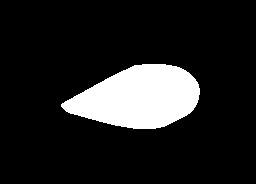
\includegraphics[width = 0.5 \textwidth]{figures/Convexhull68.png}
    \caption{Convex hull created with the canny edge detector function applied to a MRI cross-section that has been edited to remove noise outside the fish. }
    \label{fig:convexhull}
\end{figure}

As mentioned, another edge detection has been applied to the convex hull image because not the interior of the convex hull is relevant in our case but just its outer contour.

In the next step, the position of the backbone has been identified and the point itself has been excluded from the data points of the cross-section. A visualization of the resulting points for one single section can be seen in Figure \ref{fig:contours}. 
\begin{figure}
    \centering
    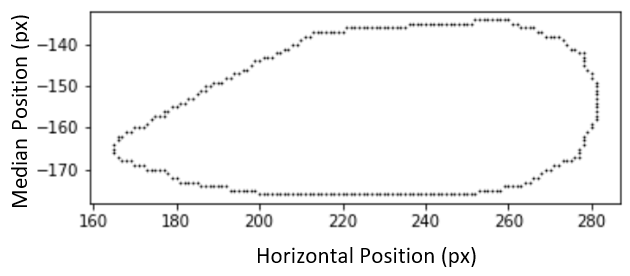
\includegraphics[width = 0.7\textwidth]{figures/contours_tight.PNG}
    \caption{Data points of the outer contour of a cross-section after having determined the convex hull without outer noise and having applied a canny edge detector to the result. }
    \label{fig:contours}
\end{figure}

The contour is still not exactly what we need for defining the distance of its points depending on $\varphi$ and the given cross-section and hence its location on the backbone. The whole contour is turned slightly because the fish was not positioned perfectly straight inside the MRI scanner. Thus, the points are turned slightly and the angle is not what one would expect. To erase this deviation from the optimal position, a rotation needs to be executed. The way to determine the angle for that same rotation is based on the first steps of a principal component analysis (PCA). The reason for applying a PCA is normally the reduction of dimensions by getting rid of dimensions that are not highly informative. To achieve this, a projection from a higher dimensional space to a lower dimensional space is executed such that the variance of the projected points is maximal \cite{scriptLuxi}. We do not want to reduce dimensions in our data but rather find the principal components and the corresponding eigenvectors to approximate the fish's original axes. Obviously, a rotation does not account for a curved axis and that is probably the case in our MRI data. But still, it is a better approximation of the original fish if we rotate the points. Furthermore, in the fitting of the function to the contours the resulting asymmetry gets wiped out because of the function's symmetry. Therefore, we follow the first three steps of the PCA described by \citeA{scriptLuxi} to be able to rotate the contour's points accordingly. 

Primarily, the data points $p_1, p_2, ..., p_n \in \mathbb{R}^2$ have been centered by computing 
\begin{flalign}
\tilde{p_i} = p_i - \overline{p}
\end{flalign}
for $0 < i \leq n, i \in \mathbb{N}$ separately for each cross-section with $\overline{p}$ describing the average over all points.

Secondly, one computes the data matrix $X$ that has the centered data points as rows and in our case the dimension $n \times 2$. The covariance matrix $C$ then follows when calculating the dot product of $X$ with its transpose:
\begin{flalign}
C = X^T \cdot X
\end{flalign}
with $C$ of dimension $2 \times 2$. 

Calculating the eigenvectors of the covariance matrix then leads us to what we wanted: two eigenvectors that approximate the fish's main axes (depicted in Figure \ref{fig:eigenvectors}).

\begin{figure}
    \centering
    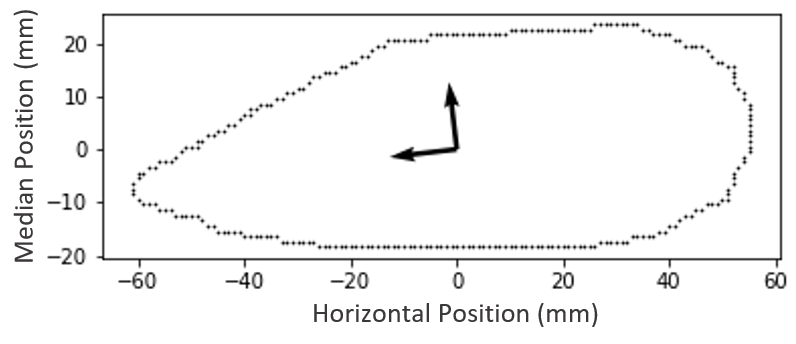
\includegraphics[width = 0.7\textwidth]{figures/eigenvectors.PNG}
    \caption{The figure shows the centered data points of the same section as are depicted in Figure \ref{fig:contours}. Additionally, the normalized eigenvectors of the covariance matrix and resulting from that the approximated fish's original axes, are marked as black arrows. }
    \label{fig:eigenvectors}
\end{figure}

As a next step, the angle $\alpha$ between the eigenvector with the larger eigenvalue, $\vec{e}$, and the horizontal axis $\vec{h}$ is calculated via 
\begin{flalign}
\alpha = \cos^{-1}\left( \frac{\vec{e} \cdot \vec{h}}{||\vec{e} \cdot \vec{h}||} \right).
\end{flalign}

Each point gets rotated around that same angle $\alpha$ in clockwise direction by applying
\begin{flalign}
\Tilde{p_i} =
\begin{pmatrix}
\cos{(-\alpha)} & -\sin{(-\alpha)}\\
\sin{(-\alpha)} & \cos{(-\alpha)}
\end{pmatrix}
\cdot \tilde{p_i}.
\end{flalign}

Having calculated these rotated points, the pre-processing of the MRI data is complete and the basis for fitting edited ellipses to the cross-sections has been created.